% ------------------------------------------------------------------------------
% TYPO3 Version 9.4 - What's New (German Version)
%
% @license	Creative Commons BY-NC-SA 3.0
% @link		https://typo3.org/help/documentation/whats-new/
% @language	German
% ------------------------------------------------------------------------------

\section{Änderungen für Integratoren}
\begin{frame}[fragile]
	\frametitle{Änderungen für Integratoren}

	\begin{center}\huge{Kapitel 2:}\end{center}
	\begin{center}\huge{\color{typo3darkgrey}\textbf{Änderungen für Integratoren}}\end{center}

\end{frame}

% ------------------------------------------------------------------------------
% #85256 - Install TYPO3 on SQLite

\begin{frame}[fragile]
	\frametitle{Änderungen für Integratoren}
	\framesubtitle{TYPO3 auf SQLite installieren(1)}

	\begin{itemize}
		\item TYPO3 unterstützt nun \href{https://www.sqlite.org}{SQLite},
			ein eigenständiges Open-Source-SQL-Datenbankmodul
		\item SQLite kann während des web-bassierten Installationsprozesses ausgewählt werden,
			wenn das PHP-Modul  "pdo\_sqlite" installiert und aktiviert ist:
	\end{itemize}

	\begin{figure}
		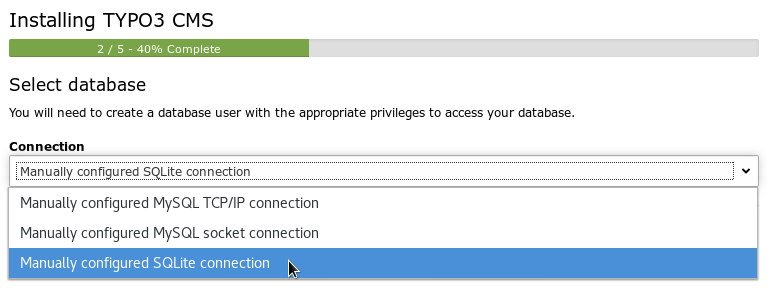
\includegraphics[width=0.65\linewidth]{ChangesForIntegrators/85256-InstallTYPO3OnSQLite.png}
	\end{figure}

\end{frame}

% ------------------------------------------------------------------------------
% #85256 - Install TYPO3 on SQLite

\begin{frame}[fragile]
	\frametitle{Änderungen für Integratoren}
	\framesubtitle{TYPO3 auf SQLite installieren (2)}

	\begin{itemize}
		\item Die Datenbank wird in einer einzigen Datei gespeichert. Das bedeutet, dass 
			TYPO3-Instanzen in PHP ausgeführt werden können.
		\item Die Verwendung von SQLite ist beispielsweise für relativ kleine TYPO3-Webseiten
			oder Test- und Entwicklungsinstanzen sinnvoll
		\item Wenn die Datei \texttt{*.sqlite} im Web-Container gespeichert wird (abhängig vom Installationstyp),
			  sollen Systemadministratoren geeignete Maßnahmen zum Schutz der Datei 
			ergreifen
	\end{itemize}

\end{frame}

% ------------------------------------------------------------------------------
% #85947 - Page based URL handling

\begin{frame}[fragile]
	\frametitle{Änderungen für Integratoren}
	\framesubtitle{Seitenbasierte URL-Handling}

	\begin{itemize}
		\item Alle Links, die im Backend und Frontend generiert werden, verwenden dieses Feld
			(wenn es gesetzt ist)
		\item Die Seitenbasierte URL-Handling erfordert eine Site Konfiguration
	\end{itemize}

	\begin{figure}
		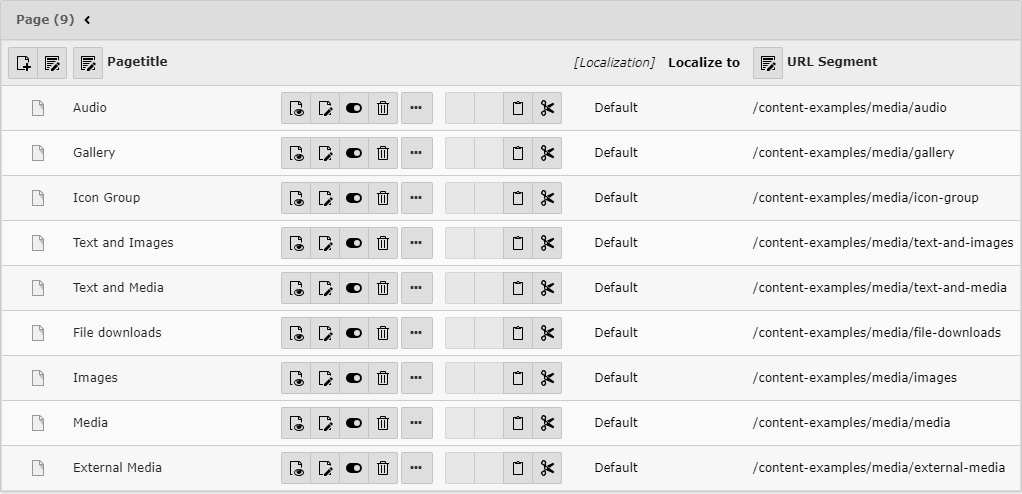
\includegraphics[width=0.7\linewidth]{ChangesForIntegrators/xxxxx-UrlSegments.png}
	\end{figure}

\end{frame}

% ------------------------------------------------------------------------------
% #84729 - New TCA type "slug"

\begin{frame}[fragile]
	\frametitle{Änderungen für Integratoren}
	\framesubtitle{Seitenbasierte URL-Handling}

	% decrease font size for code listing
	\lstset{basicstyle=\smaller\ttfamily}

	\begin{itemize}
		\item Ein neues TCA Feld wurde \texttt{slug} wurde hinzugefügt
		\item Dies bestimmt Teile eines URL-Pfades zum Generieren und Auflösen von URLs

		\begin{lstlisting}
'type' => 'slug',
  'config' => [
    'generatorOptions' => [
      'fields' => ['title', 'nav_title'],
      'fieldSeparator' => '/',
      'prefixParentPageSlug' => true
    ]
    'fallbackCharacter' => '-',
    'eval' => 'uniqueInSite'
  ]
		\end{lstlisting}
	\end{itemize}

\end{frame}

% ------------------------------------------------------------------------------
% #44297 - Interval presets for cron command of scheduler task

\begin{frame}[fragile]
	\frametitle{Änderungen für Integratoren}
	\framesubtitle{Scheduler}

	\begin{itemize}
		\item Presets wurdem zum Scheduler hinzugefügt:

			\begin{itemize}
				\item \texttt{0 9,15 * * 1-5}\tabto{3.8cm}(Mon to Fri at 9:00 and 15:00)
				\item \texttt{0 */2 * * *}\tabto{3.8cm}(every 2 hours)
				\item \texttt{*/20 * * * *}\tabto{3.8cm}(every 20 minutes)
				\item \texttt{0 7 * * 2}\tabto{3.8cm}(every Tuesday at 7:00)
			\end{itemize}

	\end{itemize}

	\begin{figure}
		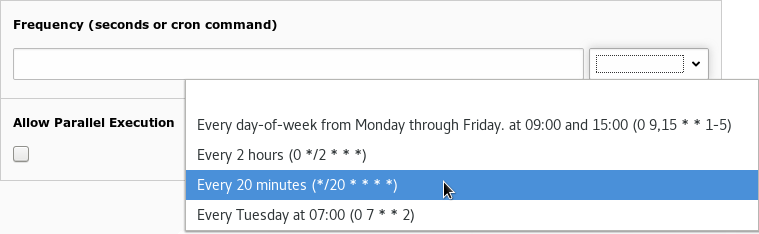
\includegraphics[width=0.80\linewidth]{ChangesForIntegrators/44297-IntervalPresetsInSchedulerTask.png}
	\end{figure}

\end{frame}

% ------------------------------------------------------------------------------
% #83476 - Load merged JS files asynchronous
% #85146 - Read environment variables in TypoScript

\begin{frame}[fragile]
	\frametitle{Änderungen für Integratoren}
	\framesubtitle{Änderungen/Verbesserungen im TypoScript (1)}

	% decrease font size for code listing
	\lstset{basicstyle=\smaller\ttfamily}

	\begin{itemize}
		\item Das Attribut \texttt{async} wird nun zum Skript-Tag der verketteten JS-Dateien
			zugewiesen, wenn im Typoscript aller Dateien das Attribut \texttt{async}
			aktiviert ist:

			\begin{lstlisting}
config.concatenateJs = 1
page = PAGE
page.includeJSFooter {
  test = path/to/file.js
  test.async = 1
}
			\end{lstlisting}

		\item Es ist nun möglich Umgebungsvariablen in TypoSkript zu lesen:

			\begin{lstlisting}
# Define default value
myConstant = defaultValue
# Enable overriding by environment variable
myConstant := getEnv(MYCONSTANT)
			\end{lstlisting}

	\end{itemize}

\end{frame}

% ------------------------------------------------------------------------------
% #85550 - Add context check for TypoScript

\begin{frame}[fragile]
	\frametitle{Änderungen für Integratoren}
	\framesubtitle{Änderungen/Verbesserungen im TypoScript (2)}

	% decrease font size for code listing
	\lstset{basicstyle=\smaller\ttfamily}

	\begin{itemize}
		\item Mit der neuen Context-API (siehe "Änderungen für Entwickler") können Integratoren
			diese auch im TypoScript verwenden

		\item Ein Beispiel dafür:

			\begin{lstlisting}
10 = TEXT
10.data = context:workspace:id
			\end{lstlisting}

		\item Die korrekte Syntax ist: \texttt{context:[aspectName]:[propertyName]}

		\item Arrays werden automatisch in kommagetrennte Listen konvertiert\newline
			\smaller(ideal zum Lesen von Details, zum Beispiel Benutzergruppen)\normalsize

	\end{itemize}

\end{frame}

% ------------------------------------------------------------------------------
% #86057 - Improved typolink / URL link generation

\begin{frame}[fragile]
	\frametitle{Änderungen für Integratoren}
	\framesubtitle{Änderungen/Verbesserungen im TypoScript (3)}

	% decrease font size for code listing
	\lstset{basicstyle=\smaller\ttfamily}

	\begin{itemize}
		\item Mit der neuen seitenbasierter Handling, der de-facto-Standard \texttt{GET}
			Parameter "L" wurde veraltet und bekam dadurch obsolete
		\item Ein neuer Parameter \texttt{typolink.language} wurde eingeführt

			\begin{lstlisting}
page.10 = TEXT
page.10.value = Link to the page with the ID in the current language
page.10.typolink.parameter = 23
page.20 = TEXT
page.20.value = Link to the page with the ID in the language 3
page.20.typolink.parameter = 23
page.20.typolink.language = 3
			\end{lstlisting}

	\end{itemize}

\end{frame}

% ------------------------------------------------------------------------------
% #85196 - Unify simulate user settings for Backend admins

\begin{frame}[fragile]
	\frametitle{Änderungen für Integratoren}
	\framesubtitle{User unter BE-Benutzereinstellungen simulieren}

	\begin{itemize}
		\item Administratorbenutzer hatten die Möglichkeit zu einem anderen Backend User
			zu wechseln ("User Settings → Simulate backend user")
		\item Diese Funktion wurde jetzt entfernt
	\end{itemize}

	\begin{figure}
		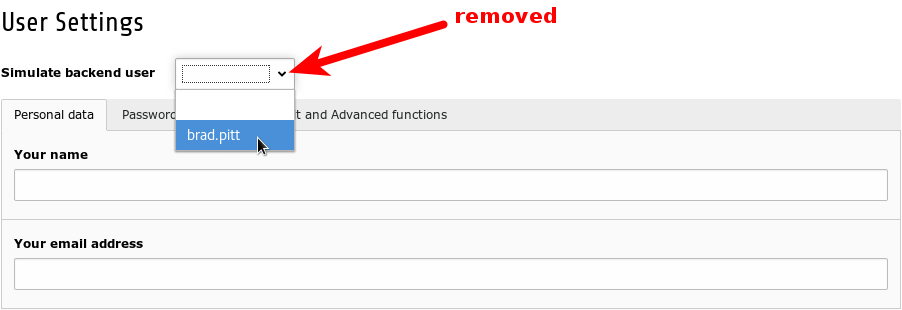
\includegraphics[width=0.80\linewidth]{ChangesForIntegrators/85196-SimulateUserRemovedForAdmins.png}
	\end{figure}

\end{frame}

% ------------------------------------------------------------------------------
% #84133 - Introduce variants

\begin{frame}[fragile]
	\frametitle{Änderungen für Integratoren}
	\framesubtitle{Bedingte Varianten in \texttt{EXT:form} (1)}

	\begin{itemize}
		\item Neues Feature für die Erweiterung "Forms": \textit{conditional variants}
		\item Die Varianten können Bedingungen enthalten und ermöglichen die Änderung der Eigenschaften eines
			Formularelements
		\item Auf diese Weise können Formelementwerte, Validierer- und Finisher-Optionen usw. 
			basierend auf Bedingungen bearbeitet werde

	\end{itemize}

\end{frame}

% ------------------------------------------------------------------------------
% #84133 - Introduce variants

\begin{frame}[fragile]
	\frametitle{Änderungen für Integratoren}
	\framesubtitle{Bedingte Varianten in \texttt{EXT:form} (2)}

	\begin{itemize}
		\item Einige typische Anwendungsfälle sind zum Beispiel:

			\begin{itemize}
				\item Formelementwerte in Abhängigkeit von der aktuellen Frontendsprache
					zu übersetzen
				\item Validatoren setzen und entfernen abhängig vom Wert eines anderen
					Formularelements
				\item Finisher-Werte festzulegen in Abhängigkeit eines Formularelements
				\item Ein Formularelement in bestimmten Finishers und auf der Übersichtsseite auszublenden. 
				\item Ganze Seiten im Workflow auszublenden abhängig vom Wert eines
					Formularelements.
				\item etc.
			\end{itemize}

		\item \href{https://docs.typo3.org/typo3cms/extensions/form}{Official documentation}
			enthält weitere Details und Beispiele

	\end{itemize}

\end{frame}

% ------------------------------------------------------------------------------
% #85355 - Support basic HTML5 fields in FormEngine

\begin{frame}[fragile]
	\frametitle{Änderungen für Integratoren}
	\framesubtitle{HTML5-Validatierung in Backend-Feldern}

	\begin{itemize}
		\item HTML5-spezifische Feldtypen und Attribute werden nun von der FormEngine
			im TYPO3-Backend gerendert.
		\item Dazu gehören E-Mails, Zahlen etc
		\item HTML-Tag-Attribute basieren auf der \texttt{eval} TCA-Konfiguration
		\item Diese Funktion wird möglicherweise die benutzerdefinierte processing JavaScript-basierte 
			Verarbeitung langfristig überflüssig machen
	\end{itemize}

\end{frame}

% ------------------------------------------------------------------------------
% #86001 - Regular Workspace cleanup tasks available via CLI commands

\begin{frame}[fragile]
	\frametitle{Änderungen für Integratoren}
	\framesubtitle{Workspace-CLI-Befehle}

	% decrease font size for code listing
	\lstset{basicstyle=\small\ttfamily}

	\begin{itemize}
		\item TYPO3 unterstützt jetzt zwei neue Symfony-basierte CLA-Befehle um reguläre
			Aufgaben auszulösen:

			\begin{itemize}

				\item \texttt{workspace:autopublish}\newline
					Sucht nach Workspaces, die für die automatische Veröffentlichung konfiguriert
					sind und führt einen Veröffentlichungs- / Austauschprozess durch.
					\newline

				\item \texttt{cleanup:previewlinks}\newline
					Entfernt von der Datenbank abgelaufene Vorschaulinks, die in sys\_preview
					gespeichert sind.

			\end{itemize}

		\item Ein Beispiel für die Ausführung:

			\begin{lstlisting}
$ typo3/sysext/core/bin/typo3 workspace:autopublish
			\end{lstlisting}

	\end{itemize}

\end{frame}

% ------------------------------------------------------------------------------
% #81430 - Improve TS Template module information on root level list

\begin{frame}[fragile]
	\frametitle{Änderungen für Integratoren}
	\framesubtitle{TypoScript-Modulinformationen}

	\begin{itemize}
		\item Überblick über TypoScript-Vorlagen auf der root-Seite wurde überarbeitet
		\item Die HTML-Ausgabe verwendet jetzt Fluid Vorlagen
		\item Zu den angezeigten Informationen gehören der Seitenname, der Vorlagenname 
			 (mit direktem Link zum Bearbeiten des TypoScript-Datensatzes), der Status 
			 (über das Symbol), die Stamm- oder Erweiterungsvorlage

	\end{itemize}

	\begin{figure}
		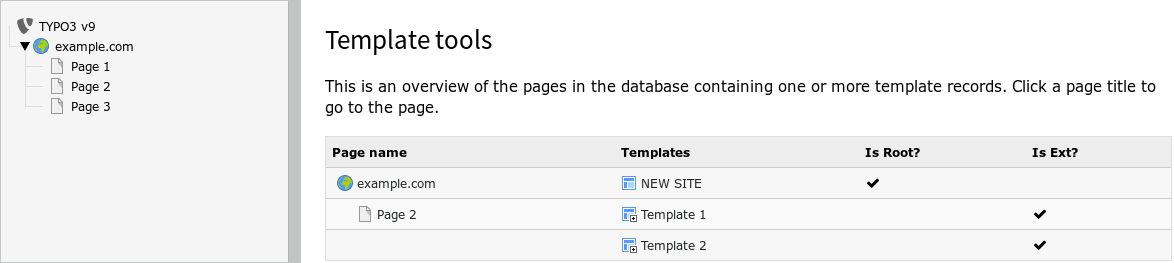
\includegraphics[width=0.80\linewidth]{ChangesForIntegrators/81430-TypoScriptModuleInformation.png}
	\end{figure}

\end{frame}

% ------------------------------------------------------------------------------
% #85393 - Only import extensions from 2015+ into EM

\begin{frame}[fragile]
	\frametitle{Änderungen für Integratoren}
	\framesubtitle{Extension Manager}

	\begin{itemize}
		\item Erweiterungen, die älter als 10. November 2015 sind (TYPO3 v7 LTS) sind vom
			Import der Erweiterungsliste ausgeschlossen
		\item Dies reduziert die Datenbanktabellengröße um ca. 75%
	\end{itemize}

\end{frame}

% ------------------------------------------------------------------------------
